\documentclass[12pt]{article}

%%%%%%%%%%%%%%%%%%%%%%%%%%%%%%%%%%%%%%%%%%%%%%%%%%%%%%%%%%%%%%%%%%%%%%%%%%%%%%%%%%%%%%%%%%%%%%%%%%%%
% Math
\usepackage{fancyhdr} 
\usepackage{amsfonts}
\usepackage{amsmath}
\usepackage{amssymb}
\usepackage{amsthm}
%\usepackage{dsfont}

%%%%%%%%%%%%%%%%%%%%%%%%%%%%%%%%%%%%%%%%%%%%%%%%%%%%%%%%%%%%%%%%%%%%%%%%%%%%%%%%%%%%%%%%%%%%%%%%%%%%
% Macros
\usepackage{calc}

%%%%%%%%%%%%%%%%%%%%%%%%%%%%%%%%%%%%%%%%%%%%%%%%%%%%%%%%%%%%%%%%%%%%%%%%%%%%%%%%%%%%%%%%%%%%%%%%%%%%
% Commands and Custom Variables	
\newcommand{\problem}[1]{\hspace{-4 ex} \large \textbf{Problem #1} }
%\let\oldemptyset\emptyset
%\let\emptyset\varnothing
\newcommand{\norm}[1]{\left\lVert#1\right\rVert}
\newcommand{\sint}{\text{s}\kern-5pt\int}
\newcommand{\powerset}{\mathcal{P}}
\renewenvironment{proof}{\hspace{-4 ex} \emph{Proof}:}{\qed}
\newcommand{\solution}{\textit{Solution}:\bigbreak}
\newcommand{\RR}{\mathbb{R}}
\newcommand{\NN}{\mathbb{N}}
\newcommand{\QQ}{\mathbb{Q}}
\newcommand{\ZZ}{\mathbb{Z}}
\newcommand{\CC}{\mathbb{C}}
\newcommand{\VV}{\mathbb{V}}
\newcommand{\FF}{\mathbb{F}}
\renewcommand{\Re}{\operatorname{Re}}
\renewcommand{\Im}{\operatorname{Im}}

\newcommand{\editnote}[1]{\textcolor{red}{\textbf{\MakeUppercase{#1}}}}


%%%%%%%%%%%%%%%%%%%%%%%%%%%%%%%%%%%%%%%%%%%%%%%%%%%%%%%%%%%%%%%%%%%%%%%%%%%%%%%%%%%%%%%%%%%%%%%%%%%%
%page
\usepackage[margin=1in]{geometry}
\usepackage{setspace}
%\doublespacing
\allowdisplaybreaks
\pagestyle{fancy}
\fancyhf{}
\rhead{Shaw \space \thepage}
\setlength\parindent{0pt}
\usepackage{color}

%%%%%%%%%%%%%%%%%%%%%%%%%%%%%%%%%%%%%%%%%%%%%%%%%%%%%%%%%%%%%%%%%%%%%%%%%%%%%%%%%%%%%%%%%%%%%%%%%%%%
%Code
\usepackage{listings}
\usepackage{courier}
\lstset{
	language=Python,
	showstringspaces=false,
	formfeed=newpage,
	tabsize=4,
	commentstyle=\itshape,
	basicstyle=\ttfamily,
}

%%%%%%%%%%%%%%%%%%%%%%%%%%%%%%%%%%%%%%%%%%%%%%%%%%%%%%%%%%%%%%%%%%%%%%%%%%%%%%%%%%%%%%%%%%%%%%%%%%%%
%Images
\usepackage{graphicx}
\graphicspath{ {images/} }
\usepackage{float}

%tikz
\usepackage[utf8]{inputenc}
%\usepackage{pgfplots}
%\usepgfplotslibrary{groupplots}

%%%%%%%%%%%%%%%%%%%%%%%%%%%%%%%%%%%%%%%%%%%%%%%%%%%%%%%%%%%%%%%%%%%%%%%%%%%%%%%%%%%%%%%%%%%%%%%%%%%%
%Hyperlinks
%\usepackage{hyperref}
%\hypersetup{
%	colorlinks=true,
%	linkcolor=blue,
%	filecolor=magenta,      
%	urlcolor=cyan,
%}

\begin{document}
	\thispagestyle{empty}
	
	\begin{flushright}
		Sage Shaw \\
		m567 - Fall 2018 \\
		\today
	\end{flushright}
	
\begin{center}{\large \textbf{Homework 1}}\end{center}
\bigbreak

\hspace{-.5 ex}\problem{1} We assume that for a given step size $h$ the error is approximately $e(h) \approx Ch^p$. Given two step sizes $h_1, h_2$ and their corresponding errors $e_1=e(h_1), e_2=e(h_2)$ we have that $e_1 \approx Ch_1^p$ and $e_2 \approx Ch_2^p$. This gives us
\begin{align*}
	\frac{e_2}{e_1} &\approx \frac{h_2^p}{h_1^p} \\
	\log \left( \frac{e_2}{e_1} \right) &\approx p\log \left( \frac{h_2}{h_1} \right) \\
	\frac{\log \left( \frac{e_2}{e_1} \right) }{\log \left( \frac{h_2}{h_1} \right)} &\approx p \text{.}
\end{align*}
We will call this approximation $p_\text{approx}$ in the tables below and will use the step size and error for its row as $e_2$ and $h_2$ respectively, and the step size and error from the previous row as $h_1$ and $e_1$ respectively. The first table is roughly first order, the second table is roughly second order, and the third table is roughly fourth order.

\begin{center}
	\begin{tabular}{|c|c|c|}
		\hline
		$h$&$e(h)$&$p_\text{approx}$\\ \hline
		0.0078125&0.020844&-\\ \hline
		0.0039062&0.011118&0.90673\\ \hline
		0.0019531&0.0053455&1.0565\\ \hline
		0.00097656&0.0027049&0.98275\\ \hline
		0.00048828&0.0013469&1.0059\\ \hline
	\end{tabular}
\end{center}
\begin{center}
	\begin{tabular}{|c|c|c|}
		\hline
		$h$&$e(h)$&$p_\text{approx}$\\ \hline
		0.0078125&0.0019059&-\\ \hline
		0.0039062&0.00043086&2.1452\\ \hline
		0.0019531&0.00010318&2.0621\\ \hline
		0.00097656&2.6007e-05&1.9882\\ \hline
		0.00048828&6.5716e-06&1.9846\\ \hline
	\end{tabular}
\end{center}
\begin{center}
	\begin{tabular}{|c|c|c|}
		\hline
		$h$&$e(h)$&$p_\text{approx}$\\ \hline
		1&0.013829&-\\ \hline
		0.5&0.0018805&2.8785\\ \hline
		0.25&0.00013742&3.7745\\ \hline
		0.125&8.917e-06&3.9459\\ \hline
		0.0625&5.6252e-07&3.9866\\ \hline
		0.03125&3.5239e-08&3.9967\\ \hline
		0.015625&2.2037e-09&3.9992\\ \hline
		0.0078125&1.3775e-10&3.9998\\ \hline
		0.0039062&8.6098e-12&3.9999\\ \hline
	\end{tabular}
\end{center}


%%%%%%%%%%%%%%%%%%%%%%%%%%%%%%%%%%%%%%%%%%%%%%%%%%%%%%%%%%%%%%%%%%%%%%%%%%%%%%%%%%%%%%%%%%%%%%%%%%%%
\problem{2(a)} Show that if we assume a uniform grid, the stencil we obtain for the approximation of $u^{\prime\prime}(x_{j+1/2})$ at the cell centers $x_{j+1/2}$ is essentially the same second order approximation we obtained in class for $u^{\prime\prime}(x_j)$ on a vertex centered grid. \bigbreak

\solution
Assuming a uniform grid with spacing $h$, we know that $x_{j+3/2}-x_{j+1/2} = x_{j+1/2}-x_{j-1/2} = h$. Then
\begin{align*}
	u^{\prime\prime}(x_{j+1/2}) &\approx \frac{1}{x_{j+1} - x_j} \left[ \frac{u(x_{j+3/2}) - u(x_{j+1/2})}{x_{j+3/2} - x_{j+1/2}} - \frac{u(x_{j+1/2}) - u(x_{j-1/2})}{x_{j+1/2} - x_{j-1/2}} \right] \\
	 &= \frac{1}{h} \left[ \frac{u(x_{j+3/2}) - u(x_{j+1/2})}{h} - \frac{u(x_{j+1/2}) - u(x_{j-1/2})}{h} \right] \\
	 &= \frac{1}{h^2} \left( u(x_{j+3/2}) - 2u(x_{j+1/2}) + u(x_{j-1/2}) \right) \text{.}
\end{align*}
These are the same weights as our three point stencil for the vertex centered approach.
\bigbreak


%%%%%%%%%%%%%%%%%%%%%%%%%%%%%%%%%%%%%%%%%%%%%%%%%%%%%%%%%%%%%%%%%%%%%%%%%%%%%%%%%%%%%%%%%%%%%%%%%%%%
\problem{2(b)} Show that the techniques differ on non-equispaced grids. 

\solution
Let $x_0 = 0, x_1 = 1, x_2 = \frac{7}{4}, \text{ and } x_3 = 3$.  Then by convention $x_{1/2} = \frac{1}{2}, x_{3/2} = \frac{11}{8}, \text{ and } x_{5/2} = \frac{19}{8}$. These points can be seen in the plot below.
\begin{figure}[H]
	%\caption{Equispaced points}
	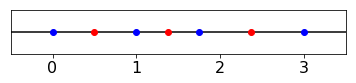
\includegraphics[width=0.4\textwidth]{unequal_points}
	\centering
\end{figure}

Our finite volume-approximation then gives us
\begin{align*}
	u^{\prime\prime}(x_{3/2}) &\approx \frac{1}{x_{2} - x_1} \left[ \frac{u(x_{5/2}) - u(x_{3/2})}{x_{5/2} - x_{3/2}} - \frac{u(x_{3/2}) - u(x_{1/2})}{x_{3/2} - x_{1/2}} \right] \\
	&= \frac{4}{3} \left[ \frac{u(x_{5/2}) - u(x_{3/2})}{1} - \frac{u(x_{3/2}) - u(x_{1/2})}{5/8} \right] \\
	&= \frac{4}{15} \left( 5u(x_{5/2}) - 5(x_{3/2}) - 8u(x_{3/2}) + 8u(x_{1/2}) \right) \\
	&= \frac{4}{15} \left[ 5u(x_{5/2}) - 13u(x_{3/2}) + 8u(x_{1/2}) \right] \\
	&\approx 1.333u(x_{5/2}) - 3.467u(x_{3/2}) + 1.067u(x_{1/2}) \text{.}
\end{align*}

However, our FD weights are given by Fornberg's Algorithm as
$$
u^{\prime\prime}(x_{j+1/2}) \approx 1.219u(x_{5/2}) - 2.286u(x_{3/2}) + 1.067u(x_{1/2})
$$
which are clearly different.
\bigbreak


%%%%%%%%%%%%%%%%%%%%%%%%%%%%%%%%%%%%%%%%%%%%%%%%%%%%%%%%%%%%%%%%%%%%%%%%%%%%%%%%%%%%%%%%%%%%%%%%%%%%
\problem{3(a)} Here is the Python (version 3.x) code that approximates the first and second derivatives of the function, given a sampling of the function over a uniform grid, as well as the first and second derivatives at the end points. 
\begin{lstlisting}
############################################################
#
# a and b are the end points
# N+1 is the number of points including the endpoints
# foo is either a function, or a list of function values
# dfa and dfb are the first derivatives at a and b 
# 		respectively
# d2fa and d2fb are the second derivatives at a and b 
# 		respectively
# 
# returns the first and second derivatives at the points
#
############################################################
def hermite(a, b, N, foo, dfa, dfb, d2fa, d2fb):
	xs = np.linspace(a,b,N+1)
	if callable(foo):
		fs = foo(xs)
	else:
		assert len(foo)==N+1
		fs = foo
	h = (b-a)/N
	inner_N = N-1
	
	D1 = sp.diags( [[1]*(inner_N-1), 
					[4]*(inner_N),
					[1]*(inner_N-1) ],
					[-1,0,1], format='csr')
	f1 = [3/h*(-f0+f2) for f0, f2 in zip(fs[:-2], fs[2:] )]
	f1[0] -= dfa
	f1[-1] -= dfb
	fd1 = np.zeros(N+1)
	fd1[0], fd1[-1] = dfa, dfb
	fd1[1:-1] = spsolve(D1, f1)
	
	D2 = sp.diags( [[1]*(inner_N-1),
					[10]*(inner_N),
					[1]*(inner_N-1) ], 
					[-1,0,1], format='csr')
	f2 = [ 12/(h**2) * (f0 - 2*f1 + f2) for
		 	f0, f1, f2 in zip( fs[:-2], fs[1:-1], fs[2:] )]
	f2[0] -= d2fa
	f2[-1] -= d2fb
	fd2 = np.zeros(N+1)
	fd2[0], fd2[-1] = d2fa, d2fb
	fd2[1:-1] = spsolve(D2, f2)

return fd1, fd2
\end{lstlisting}
\bigbreak


%%%%%%%%%%%%%%%%%%%%%%%%%%%%%%%%%%%%%%%%%%%%%%%%%%%%%%%%%%%%%%%%%%%%%%%%%%%%%%%%%%%%%%%%%%%%%%%%%%%%
\problem{3(b)} Applied to the function $x^2e^{-x}$ over the interval $[0,1]$ the errors for the $L_2$ norm of first and second derivatives approximated at $N$ points for $N=8$ and doubling until $N=256$ can be seen in the table and plots below.\\

\begin{center}
	\begin{tabular}{|c|c|c|c|c|}
		\hline
		$h$&$f^\prime$ erorr&$f^\prime$ erorr order&$f^{\prime\prime}$ erorr&$f^{\prime\prime}$ erorr order\\ \hline
		0.125&2.8053e-05&-&3.1002e-05&-\\ \hline
		0.0625&3.0451e-06&3.2036&3.4432e-06&3.1706\\ \hline
		0.03125&2.9927e-07&3.347&3.4287e-07&3.328\\ \hline
		0.015625&2.7916e-08&3.4223&3.2209e-08&3.4121\\ \hline
		0.0078125&2.5354e-09&3.4608&2.936e-09&3.4556\\ \hline
		0.0039062&2.2717e-10&3.4803&2.7081e-10&3.4385\\ \hline
	\end{tabular}
\end{center}

\begin{figure}[H]
	%\caption{Equispaced points}
	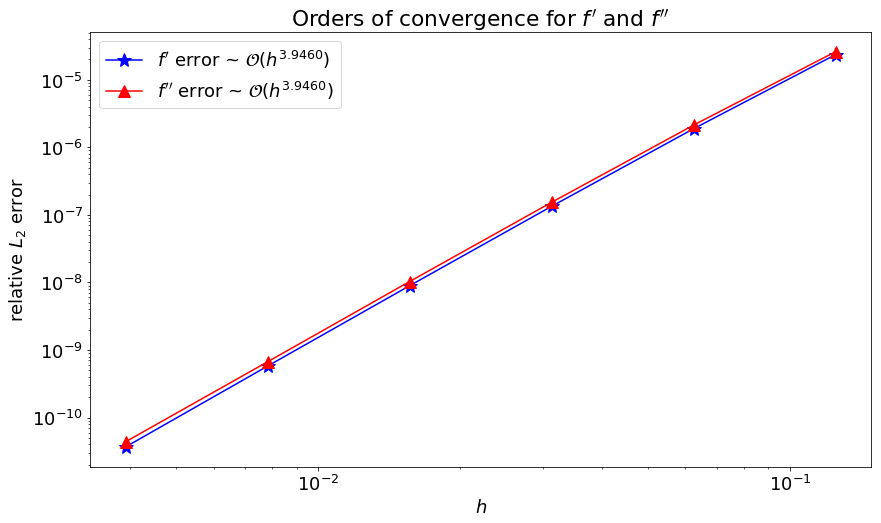
\includegraphics[width=.9\textwidth]{hw1_p3b_order_plot}
	\centering
\end{figure}

The order of accuracy appears to be roughly $\mathcal{O}(h^{3.4})$ for both methods.
\bigbreak

\problem{3(c)} Using Maple the output of the provided code can be seen in the figure below.
\begin{figure}[H]
	\caption{Maple code for error analysis of the first derivative.}
	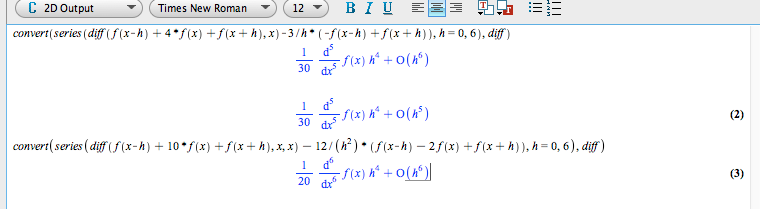
\includegraphics[width=1\textwidth]{hw1_p3c_maple}
	\centering
\end{figure}
These results are verified in Python using the package Sympy in the following code.
\begin{lstlisting}
n = 6
x0 = 0
x, h = smp.symbols('x h')
f = smp.Function('f')

right = f(x+h).series(x+h, x0=x0, n=n)
right -= f(x-h).series(x-h, x0=x0, n=n)
right *= 3/h
right = right.subs(x,x0).simplify()

left = f(x+h).series(x+h, x0=x0, n=n).diff(x) 
left += f(x-h).series(x-h, x0=x0, n=n).diff(x)
left += 4*f(x).diff(x).subs(x,x0)
left = left.subs(x,x0).simplify()

err = (left - right).subs(x,0).simplify()
display(err)
\end{lstlisting}
The output of the code is
$$
\frac{h^{4} \left. \frac{d^{5}}{d x^{5}} f{\left (x \right )} \right|_{\substack{ x=0 }}}{30} + O\left(h^{5}\right)
$$
confirming that the error is $\mathcal{O}(h^4)$.
\bigbreak

Similar code can be used to prove the same for the second derivative approximation.
\begin{lstlisting}
n = 7
x0 = 0
x, h = smp.symbols('x h')
f = smp.Function('f')

right = f(x+h).series(x+h, x0=x0, n=n)
right += f(x-h).series(x-h, x0=x0, n=n)
right += -2*f(x)
right *= 12/(h**2)
right = right.subs(x,x0).simplify()

left = f(x+h).series(x+h, x0=x0, n=n).diff(x,2) 
left += f(x-h).series(x-h, x0=x0, n=n).diff(x,2)
left += 10*f(x).diff(x,2)
left = left.subs(x,x0).simplify()

err = (left - right).subs(x,0).simplify()
display(err)
\end{lstlisting}
The output of the above code is
$$
\frac{h^{4} \left. \frac{d^{6}}{d x^{6}} f{\left (x \right )} \right|_{\substack{ x=0 }}}{20} + O\left(h^{5}\right)
$$
confirming that the error is $\mathcal{O}(h^4)$.
\bigbreak

%%%%%%%%%%%%%%%%%%%%%%%%%%%%%%%%%%%%%%%%%%%%%%%%%%%%%%%%%%%%%%%%%%%%%%%%%%%%%%%%%%%%%%%%%%%%%%%%%%%%
\problem{4(a)} The weights for the equispaced points that approximate the derivative at $x=0$ and $x=-1+\tfrac{3}{14}$ are given in the table below and seen in figure (\ref{equ_weights}). 
\begin{center}
	\begin{tabular}{|c|c|c|}
		\hline
		$x$&weights for $z=0.00$&weights for $z=-\tfrac{11}{14}$\\ \hline
		-1&-0.00029138&0.097975\\ \hline
		-0.85714&0.0047591&-6.2847\\ \hline
		-0.71429&-0.037121&1.4593\\ \hline
		-0.57143&0.18561&16.859\\ \hline
		-0.42857&-0.68056&-34.022\\ \hline
		-0.28571&2.0417&52.402\\ \hline
		-0.14286&-6.125&-63.599\\ \hline
		0&-1.1879e-14&60.934\\ \hline
		0.14286&6.125&-45.866\\ \hline
		0.28571&-2.0417&26.818\\ \hline
		0.42857&0.68056&-11.939\\ \hline
		0.57143&-0.18561&3.912\\ \hline
		0.71429&0.037121&-0.88992\\ \hline
		0.85714&-0.0047591&0.12559\\ \hline
		1&0.00029138&-0.0082855\\ \hline
	\end{tabular}
\end{center}

\begin{figure}[H]
	\caption{Weights for equispaced points}
	\label{equ_weights}
	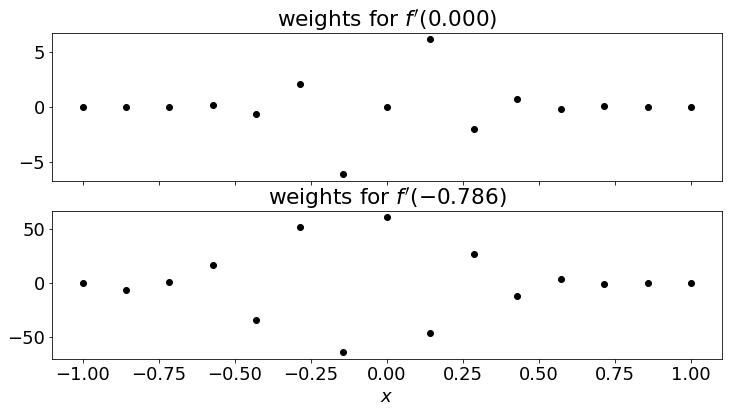
\includegraphics[width=.9\textwidth]{hw1_p4b_equi_weights}
	\centering
\end{figure}

The weights for the Chebyshev points that approximate the derivative at $x=0$ and $x=-1+\tfrac{3}{14}$ are given in the table below and seen in figure (\ref{cheb_weights}). 
\begin{center}
	\begin{tabular}{|c|c|c|}
		\hline
		$x$&weights for $z=0.00$&weights for $z=-\tfrac{11}{14}$\\ \hline
		-1&-0.5&-2.348\\ \hline
		-0.97493&1.0257&5.3308\\ \hline
		-0.90097&-1.1099&-8.8652\\ \hline
		-0.78183&1.279&1.6842\\ \hline
		-0.62349&-1.6039&5.945\\ \hline
		-0.43388&2.3048&-2.7777\\ \hline
		-0.22252&-4.494&1.7425\\ \hline
		-6.1232e-17&-1.2212e-15&-1.2515\\ \hline
		0.22252&4.494&0.97637\\ \hline
		0.43388&-2.3048&-0.8077\\ \hline
		0.62349&1.6039&0.69933\\ \hline
		0.78183&-1.279&-0.62887\\ \hline
		0.90097&1.1099&0.58455\\ \hline
		0.97493&-1.0257&-0.56005\\ \hline
		1&0.5&0.2761\\ \hline
	\end{tabular}
\end{center}

\begin{figure}[H]
	\caption{Weights for the Chebyshev points}
	\label{cheb_weights}
	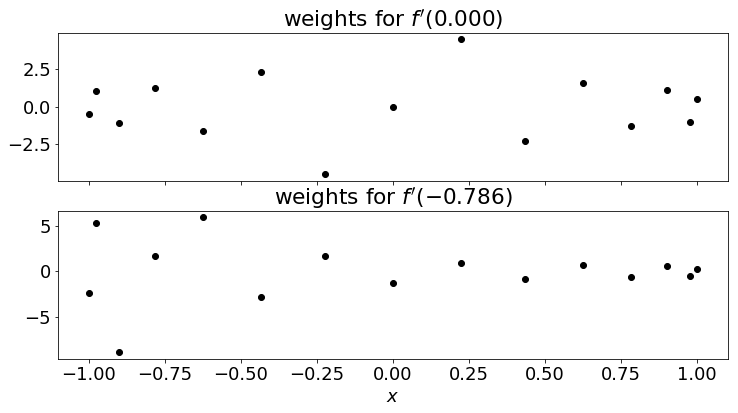
\includegraphics[width=.9\textwidth]{hw1_p4b_cheb_weights}
	\centering
\end{figure}

The weights for the Legendre points that approximate the derivative at $x=0$ and $x=-1+\tfrac{3}{14}$ are given in the table below and seen in figure (\ref{lege_weights}). 
\begin{center}
	\begin{tabular}{|c|c|c|}
		\hline
		$x$&weights for $z=0.00$&weights for $z=-\tfrac{11}{14}$\\ \hline
		-0.98799&-0.06093&-0.21617\\ \hline
		-0.93727&0.2192&1.1672\\ \hline
		-0.84821&-0.45417&-10.026\\ \hline
		-0.72442&0.78988&9.3704\\ \hline
		-0.57097&-1.3026&-0.19053\\ \hline
		-0.39415&2.2352&-0.26132\\ \hline
		-0.20119&-4.8186&0.30643\\ \hline
		0&4.4949e-16&-0.28052\\ \hline
		0.20119&4.8186&0.23726\\ \hline
		0.39415&-2.2352&-0.19042\\ \hline
		0.57097&1.3026&0.14473\\ \hline
		0.72442&-0.78988&-0.10234\\ \hline
		0.84821&0.45417&0.064645\\ \hline
		0.93727&-0.2192&-0.033001\\ \hline
		0.98799&0.06093&0.0094389\\ \hline
	\end{tabular}
\end{center}

\begin{figure}[H]
	\caption{Weights for Legendre points}
	\label{lege_weights}
	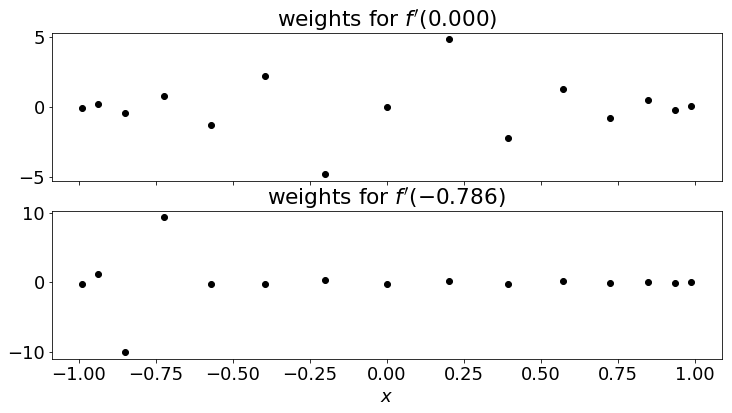
\includegraphics[width=.9\textwidth]{hw1_p4b_lege_weights}
	\centering
\end{figure}
\bigbreak

\textit{Comparison}: In the equispaced points, the weights closer to the point at which we were approximating the derivative were larger, and grew smaller as we moved farther away. The Chebyshev points seemed to weight the points more equally. The Legendre points were similar to the equispaced points when approximating $f^\prime(0)$ but heavily weighted a few negative points for the approximation of $f^\prime(-\tfrac{11}{14})$. It should also be noted that all the weights for the approximation of $f^\prime(0)$ in all three point sets had rotational symmetry about $0$. That is that if $w(x_i)$ is the weight at $x_i$ then $w(-x_i) = -w(x_i)$.
\bigbreak


%%%%%%%%%%%%%%%%%%%%%%%%%%%%%%%%%%%%%%%%%%%%%%%%%%%%%%%%%%%%%%%%%%%%%%%%%%%%%%%%%%%%%%%%%%%%%%%%%%%%
\problem{4(b)} For the function $f(x)=e^{-\cos(2(x-.2))}$, Sympy was used to formulate the derivative and compare it to the error in the approximation using all three point sets. The results are shown in the table below.

\begin{center}
	\begin{tabular}{|c|c|c|}
		\hline
		Points&Error in $f^\prime(0)$&Error in $f^\prime(-\tfrac{11}{14})$\\ \hline
		Equispaced&1.622e-07&3.9239e-06\\ \hline
		Chebyshev&3.3263e-06&1.2269e-06\\ \hline
		Legendre&1.817e-06&2.5066e-07\\ \hline
	\end{tabular}
\end{center}
From these errors none of the point sets seem particularly better than the rest. Using any would be fine.
\bigbreak

%%%%%%%%%%%%%%%%%%%%%%%%%%%%%%%%%%%%%%%%%%%%%%%%%%%%%%%%%%%%%%%%%%%%%%%%%%%%%%%%%%%%%%%%%%%%%%%%%%%%
\problem{5(a)} The periodic sinc function is defined as
$$
S_N(t) = \begin{cases}
\frac{1}{N} \sin \left(\frac{N}{2}t \right) \cot \left( \frac{1}{2}t \right) & \text{ if } N \text{ even}\\
\frac{1}{N} \sin \left(\frac{N}{2}t \right) \csc \left(\frac{1}{2}t \right) & \text{ if } N \text{ odd .}
\end{cases}
$$
Let $x_j = \frac{2\pi j}{N}, j=0,1,...,N-1$ and show that $S_N(0)=1$ and that \\$S_N(x_j-x_k)=0$ when $k\neq j$.
\bigbreak

\begin{proof} If $k \neq j$ then $\vert j - k \vert < N$ and
	\begin{align*}
		x_j - x_k &= \frac{2\pi j}{N} - \frac{2\pi k}{N} \\
		&= \frac{2\pi}{N} (j-k) \\
		&= \frac{2\pi}{N}z
	\end{align*}
	where $z$ is a non-zero integer such that $\vert z \vert < N$. There are now four cases to consider. 
	\bigbreak
	
	\textbf{Case 1}: $N$ is even and $z=0$. \\
	\textbf{Case 2}: $N$ is even and $z \neq 0$. \\
	\textbf{Case 3}: $N$ is odd and $z=0$. \\
	\textbf{Case 4}: $N$ is odd and $z \neq 0$. \\
	We will consider each individually.
	\bigbreak
	
	Note the angle multiple identity
	\begin{align}
	\sin(n \theta) &= \sum_{k=0}^n {n \choose k} \cos^k(\theta) + \sin^{n-k}(\theta) \sin(\tfrac{n-k}{2}\pi) \nonumber \\
	\sin(n \theta) &= \sum_{k=0}^{n-1} {n \choose k} \cos^k(\theta) + \sin^{n-k}(\theta) \sin(\tfrac{n-k}{2}\pi) \text{.} \label{trig_ident}
	\end{align}
	
	\textbf{Case 1}: Suppose that $N$ is even and $z=0$. \bigbreak
	Then
	$$
	S_N(0) = \frac{1}{N} \sin \left(0 \right) \cot \left( 0 \right)
	$$
	but since $\cot(0)$ is undefined we have a discontinuity. It turns out that this is a removable discontinuity as seen by
	\begin{align*}
		\lim_{x \to 0}S_N \left( \tfrac{N}{2}x \right) &= \lim_{x \to 0} \frac{1}{N} \sin \left(\pi \tfrac{N}{2}x \right) \cot \left( \tfrac{\pi}{N}\tfrac{N}{2}x \right) \\
		&= \lim_{x \to 0} \frac{1}{N} \sin \left(N \tfrac{\pi}{2}x \right) \cot \left( \tfrac{\pi}{2}x \right) \\
		&= \lim_{x \to 0} \frac{1}{N}  \cot \left( \tfrac{\pi}{2}x \right) \sum_{k=0}^{N-1} {N \choose k} \cos^k(\tfrac{\pi}{2}x) \sin^{N-k}(\tfrac{\pi}{2}x) \sin(\tfrac{N-k}{2}\pi) \text{ by }(\ref{trig_ident})\\
		&= \lim_{x \to 0} \frac{1}{N} \sum_{k=0}^{N-1} {N \choose k} \cos^{k+1}(\tfrac{\pi}{2}x) \sin^{N-k-1}(\tfrac{\pi}{2}x) \sin(\tfrac{N-k}{2}\pi) \\
		&= \frac{1}{N} {N \choose N-1} \cos^{N}(0)\sin^{0}(0) \sin(\tfrac{1}{2}\pi) \\
		&= \frac{1}{N} N (1^{N})(0^0)(1) \\
		&= 1 \text{.}
	\end{align*}
	\textbf{End of case 1.}
	\bigbreak
	
	Note that if $N$ is even then
	\begin{align}
	S_N(x_j - x_k) &= S_N\left( \frac{2\pi}{N}z \right) \nonumber \\
	&= \frac{1}{N} \sin \left(\frac{N}{2}\frac{2\pi}{N}z \right) \cot \left( \frac{1}{2}\frac{2\pi}{N}z \right) \nonumber \\
	S_N(z) &= \frac{1}{N} \sin \left(\pi z \right) \cot \left( \frac{\pi}{N}z \right) \label{N_even} \text{ for }N \text{ even.}
	\end{align}
	
	%\textbf{Case 2}: $N$ is even and $z = \pm \frac{N}{2}$. \\
	\textbf{Case 2}: $N$ is even and $z \neq 0$. \\
	Then since $z \neq 0$ and $-\pi < \frac{\pi}{N}z < \pi$ we know that $\cot(\tfrac{\pi}{N}z) \in \RR$ and thus
	\begin{align*}
		S_N(z) &= \frac{1}{N} \sin \left(\pi z \right) \cot \left( \frac{\pi}{N}z \right) \text{\ \ \ \ \ by (\ref{N_even})}\\
		&= 0 \text{.}
	\end{align*}
	\textbf{End of case 2.}
	\bigbreak
	
	Note that if $N$ is odd then
	\begin{align}
	S_N(x_j - x_k) &= S_N\left( \frac{2\pi}{N}z \right) \nonumber \\
	&= \frac{1}{N} \sin \left(\frac{N}{2}\frac{2\pi}{N}z \right) \csc \left( \frac{1}{2}\frac{2\pi}{N}z \right) \nonumber \\
	S_N(z) &= \frac{1}{N} \sin \left(\pi z \right) \csc \left( \frac{\pi}{N}z \right) \label{N_odd} \text{ for }N \text{ odd.}
	\end{align}
	\bigbreak
	
	\textbf{Case 3}: $N$ is odd and $z=0$. \\
	Then
	$$
	S_N(0) = \frac{1}{N} \sin \left(0 \right) \csc \left( 0 \right)
	$$
	but since $\csc(0)$ is undefined we have a discontinuity. It turns out that this is a removable discontinuity as seen by
	\begin{align*}
		\lim_{x \to 0}S_N \left( \tfrac{N}{2}x \right) &= \lim_{x \to 0} \frac{1}{N} \sin \left(\pi \tfrac{N}{2}x \right) \csc \left( \tfrac{\pi}{N}\tfrac{N}{2}x \right) \\
		&= \lim_{x \to 0} \frac{1}{N} \sin \left(N \tfrac{\pi}{2}x \right) \csc \left( \tfrac{\pi}{2}x \right) \\
		&= \lim_{x \to 0} \frac{1}{N}  \csc \left( \tfrac{\pi}{2}x \right) \sum_{k=0}^{n-1} {N \choose k} \cos^k(\tfrac{\pi}{2}x) \sin^{N-k}(\tfrac{\pi}{2}x) \sin(\tfrac{N-k}{2}\pi) \text{ by }(\ref{trig_ident})\\
		&= \lim_{x \to 0} \frac{1}{N} \sum_{k=0}^{N-1} {N \choose k} \cos^{k}(\tfrac{\pi}{2}x) \sin^{N-k-1}(\tfrac{\pi}{2}x) \sin(\tfrac{N-k}{2}\pi) \\
		&= \frac{1}{N} {N \choose N-1} \cos^{N-1}(0)\sin^{0}(0) \sin(\tfrac{1}{2}\pi) \\
		&= \frac{1}{N} N (1^{n-1})(0^0)(1) \\
		&= 1 \text{.}
	\end{align*}
	
	\textbf{End of case 3.}
	\bigbreak
	
	\textbf{Case 4}: $N$ is odd and $z\neq 0$. \\
	Then since $z \neq 0$ and $-\pi < \frac{\pi}{N}z < \pi$ we know that $\csc(\tfrac{\pi}{N}z) \in \RR$ and thus
	\begin{align*}
		S_N(z) &= \frac{1}{N} \sin \left(\pi z \right) \csc \left( \frac{\pi}{N}z \right) \tag{\text{by (\ref{N_even})}}\\
		&= 0 \text{.}
	\end{align*}	
	
	\textbf{End of case 4.}
	\bigbreak
	
	Thus we conclude that $S_N(0)=1$ and that if $j \neq k$ then $S_N(x_j - x_k) = 0$.
	
\end{proof}
\bigbreak

%%%%%%%%%%%%%%%%%%%%%%%%%%%%%%%%%%%%%%%%%%%%%%%%%%%%%%%%%%%%%%%%%%%%%%%%%%%%%%%%%%%%%%%%%%%%%%%%%%%%
\problem{5(b)} For $N$ even, show that 
$$
S_N^\prime(x_k) = \begin{cases} 0 & \text{if } k=0 \\
							\frac{1}{2}(-1)^k\cot(k\pi / N), & \text{if } k \neq 0 \text{.} \end{cases}
$$
\begin{proof}
	First note that since sine and cotangent are odd functions, $S_N$ is even. Thus for any $x \in \RR$ we know that $S_N(x) = S_N(-x)$. Then we have that
	\begin{align*}
		S_N^\prime(0) &= \lim_{h \to 0} \frac{S_N(0+h) - S_N(0-h)}{2h} \\
			&= \lim_{h \to 0} \frac{S_N(h) - S_N(-h)}{2h} \\
			&= \lim_{h \to 0} \frac{S_N(h) - S_N(h)}{2h} \text{\ \ \ \ (since it's even)}\\
			&= \lim_{h \to 0} \frac{0}{2h} \\
			&= \lim_{h \to 0} 0 \\
			&= 0 \text{.}
	\end{align*}
	Thus $S_N^\prime(x_0) = 0$.\bigbreak
	
	In general for $N$ even,
	\begin{align*}
		S_N^\prime(t) &= \frac{d}{dt} \bigg[\frac{1}{N} \sin \left(\frac{N}{2}t \right) \cot \left( \frac{1}{2}t \right) \bigg] \\
		&= \frac{1}{N} \bigg[ \frac{N}{2}\cos\left(\frac{N}{2}t \right)\cot \left( \frac{1}{2}t \right) + 
			\sin \left(\frac{N}{2}t \right) \left(\tfrac{-1}{2} \right) \csc^2\left( \frac{1}{2}t \right) \bigg] \\
		&= \frac{1}{2}\cos\left(\frac{N}{2}t \right)\cot \left( \frac{1}{2}t \right) - 
		\frac{1}{2N}\sin \left(\frac{N}{2}t \right)  \csc^2 \left( \frac{1}{2}t \right) \text{.}
	\end{align*}
	For $0 < k < N$ we have that
	\begin{align*}
		S_N^\prime(x_k) &= S_N^\prime\left(\frac{2\pi}{N}k \right) \\
		&= \frac{1}{2}\cos\left(\frac{N}{2}\frac{2\pi}{N}k \right)\cot \left( \frac{1}{2}\frac{2\pi}{N}k \right) - 
		\frac{1}{2N}\sin \left(\frac{N}{2}\frac{2\pi}{N}k \right)  \csc^2 \left( \frac{1}{2}\frac{2\pi}{N}k \right) \\
		&= \frac{1}{2}\cos(\pi k )\cot \left( \frac{\pi k}{N} \right) - 
		\frac{1}{2N}\sin(\pi k )  \csc^2 \left( \frac{\pi k}{N} \right) \\
		&= \frac{1}{2}(-1)^k \cot \left( \frac{\pi k}{N} \right)
	\end{align*}
\end{proof}

\end{document}
